\documentclass[UTF8,titlepage]{article}
\usepackage{amsmath,amssymb,amsthm,amsfonts,amscd}
\usepackage{fontspec}
\setmainfont{Times New Roman}
\usepackage{graphicx}
\usepackage{titlesec}
\usepackage{makecell}
\usepackage{longtable}
\usepackage{xcolor}
\usepackage{tcolorbox}
\usepackage{soul}
\usepackage{adjustbox}
\usepackage{tcolorbox}
\usepackage{enumerate}
\usepackage{pdfpages}
\usepackage{float}
\usepackage{colortbl}
\usepackage{tabularx}
\usepackage{multirow}
\usepackage{pgfplots}
\numberwithin{figure}{section}
\usepackage[left=1.25in,right=1.25in,%
top=1in,bottom=1in]{geometry}
\usepackage{color}
\titleformat{\section}
  {\raggedright\LARGE\bfseries}{\thesection}{1em}{}
\title{Answer for Problem Set 5}
\author{Boyuan Zhao}
\begin{document}
\begin{center}
    {\LARGE \textbf{Answer of Problem Set 5}}\\  % 这就是你的标题
    {\normalsize Boyuan Zhao}\\  % 这就是你的名字
    {\small \today}  % 这是日期
\end{center}

\section{Problem 1. Monopoly, Oligopoly, and Perfect Competition}
\begin{enumerate}
\item Given \( c(y) = c y \), marginal cost (MC) is the derivative of the total cost with respect to y:
\[ MC = \frac{dc(y)}{dy} = c \]

The average cost (AC) is the total cost divided by y:
\[ AC = \frac{c(y)}{y} = c \]

Since \( p(Y) = a - b Y \), a firm will supply when the price is at least equal to the marginal cost. Thus, 
\[ y_i^*(p) = 
\begin{cases} 
0 & \text{if } p < c \\
\text{any positive value} & \text{if } p = c \\
\infty & \text{if } p > c 
\end{cases}
\]
For the industry with J firms,
\[ Y^*(p) = J y_i^*(p) \]
It becomes infinite for \( p > c \).

\item Given \( Y^*(p) \) is infinite for \( p > c \), the industry level production is:
\[ Y_{PC}^* = \frac{a - c}{b} \]
And the price level under perfect competition is:
\[ p_{PC}^* = c \]

\item As \( c \) increases, \( Y_{PC}^* \) decreases and \( p_{PC}^* \) increases. If \( a \) increases, \( Y_{PC}^* \) increases but \( p_{PC}^* \) remains at \( c \).

\item The monopolist's profit maximization problem is:
\[ \max_{y} \left[ (a - b y)y - c y \right] \]

The first order condition is:
\[ \frac{d}{dy} [(a - by)y - cy] = a - 2by - c = 0 \]

\item From the FOC:
\[ y_M^* = \frac{a - c}{2b} \]
Substitute into demand function:
\[ p_M^* = a - b \frac{a - c}{2b} = \frac{a + c}{2} \]

As \( a \) increases, \( y_M^* \) increases and \( p_M^* \) increases.

\item Under monopoly, output is lower and prices are higher than perfect competition.

Monopoly profit:
\[ \pi_M = (p_M^* - c) y_M^* = (\frac{a + c}{2} - c) \frac{a - c}{2b} = \frac{(a - c)^2}{4b} \]

Perfect competition profit:
\[ \pi_{PC} = (p_{PC}^* - c) y_i^*(p) = 0 \]
because price equals cost.

\item Each firm's profit maximization problem is:
\[ \max_{y_i} \left[ (a - b(y_i + y_{-i}))y_i - c y_i \right] \]

\item \[ \frac{d}{dy_i} [(a - b(y_i + y_{-i}))y_i - c y_i] = a - b(y_i + y_{-i}) - by_i - c = 0 \]

\item From FOC for firms 1 and 2:
\[ y_1^* = \frac{a - c - b y_2^*}{2b} \]
\[ y_2^* = \frac{a - c - b y_1^*}{2b} \]

Solving gives:
\[ y_1^* = y_2^* = \frac{a - c}{3b} \]

Industry production:
\[ Y_D^* = y_1^* + y_2^* = \frac{2(a - c)}{3b} \]

Price:
\[ p_D^* = a - b Y_D^* = a - \frac{2(a - c)}{3} = \frac{a + 2c}{3} \]

Profits for each firm:
\[ \pi_{i, D}^* = (p_D^* - c) y_i^* = \frac{(a - c)^2}{9b} \]

Aggregate profit:
\[ \Pi_D^* = 2 \pi_{i, D}^* = \frac{2(a - c)^2}{9b} \]

\item From our previous derivations, for perfect competition:
\[ p_{PC}^* = c \]
\[ Y_{PC}^* = \frac{a - c}{b} \]

For monopoly:
\[ p_M^* = \frac{a + c}{2} \]
\[ Y_M^* = \frac{a - c}{2b} \]

For duopoly:
\[ p_D^* = \frac{a + 2c}{3} \]
\[ Y_D^* = \frac{2(a - c)}{3b} \]

Now, let's compare:

Output: \( Y_M^* < Y_D^* < Y_{PC}^* \). Monopoly produces the least, duopoly produces more but still less than perfect competition.
Prices: \( p_M^* > p_D^* > p_{PC}^* \). Monopoly charges the highest price, duopoly charges less, and perfect competition charges the lowest price.
Profits: Monopolists have the highest profits since they charge a much higher price than marginal cost. Duopolists earn positive profits but less than monopolists. Perfect competitors earn zero profits in the long run as price equals marginal cost.

\item For \(I\) firms, a firm's profit maximization problem considering the others' output is:
\[ \max_{y_i} \left[ (a - b(y_i + (I-1)y_{-i}))y_i - c y_i \right] \]

The first order condition:
\[ \frac{d}{dy_i} [(a - b(y_i + (I-1)y_{-i}))y_i - c y_i] = a - b(y_i + (I-1)y_{-i}) - by_i - c = 0 \]

\item Given the symmetry condition \(y_i^* = y_{-i}^*\), and using the above:
\[ y_O^* = \frac{a - c}{(I+1)b} \]

Industry production:
\[ Y_O^* = I y_O^* = \frac{I(a - c)}{(I+1)b} \]
Price:
\[ p_O^* = a - b Y_O^* = \frac{1}{I+1} a+\frac{I}{I+1} c\]
Profits for each firm:
\[ \pi_{O}^* = (p_O^* - c) y_O^* = \frac{(a-c)^{2}}{(I+1)^{2} b} \]
Aggregate profit:
\[ \Pi_O^* = I \pi_{O}^* = I \frac{(a-c)^{2}}{(I+1)^{2} b}\]

\item As \(I \to \infty\):\\
\( y_O^* \to 0 \)\\ 
\( Y_O^* \to \frac{a - c}{b} = Y_{PC}^* \)\\
\( p_O^* \to c = p_{PC}^* \)\\
\( \pi_O^* \to 0 \)\\
\( \Pi_O^* \to 0 \)

The above results show that as the number of firms in an oligopoly becomes very large (approaches infinity), the oligopolistic market behaves like a perfectly competitive market.

In Bertrand competition with identical products, even two firms are enough to result in prices being driven down to marginal costs. This starkly contrasts with the Cournot model of quantity competition, where the number of firms must approach infinity to reach the perfect competition outcome.

These insights provide a foundation for understanding why, in some markets, a small number of firms may result in competitive prices, while in others, even a large number of firms may have market power.
\end{enumerate}

\section{Problem 2. Dynamic Games}

\begin{enumerate}
\item Profit Functions for Firm 1 and Firm 2

Firm 1's profit function is the sum of its profits from the West Coast and the East Coast. 

For the West Coast:
\[ \pi_{1W} = p_W(x_W) \times x_W - c x_W \]
\[ \pi_{1W} = (1-x_W) x_W - c x_W \]

For the East Coast:
\[ \pi_{1E} = p_E(x_E, x_2) \times x_E - (c-\alpha x_W) x_E \]
\[ \pi_{1E} = (1-x_E-x_2) x_E - (c-\alpha x_W) x_E \]

Thus, the total profit for Firm 1 is:
\[ \max _{x_{W}, x_{E}}\pi_1=\max _{x_{W}, x_{E}} x_{W}\left(1-x_{W}\right)-c x_{W}+x_{E}\left(1-x_{E}-x_{2}\right)-\left(c-\alpha x_{W}\right) x_{E} \]

Firm 2's profit function is:
\[ \max_{x_E,x_2}\pi_2 = \max_{x_E,x_2}(1-x_E-x_2) x_2 - c x_2 \]

\item First Order Conditions

To find the Nash Equilibrium, we'll differentiate the profit functions with respect to the respective quantities and set them to zero.

For Firm 1 with respect to \(x_W\):
\[ \frac{d\pi_1}{dx_W} = \frac{d\pi_{1W}}{dx_W} + \frac{d\pi_{1E}}{dx_W} \]

For Firm 1 with respect to \(x_E\):
\[ \frac{d\pi_1}{dx_E} = \frac{d\pi_{1E}}{dx_E} \]

For Firm 2 with respect to \(x_2\):
\[ \frac{d\pi_2}{dx_2} \]

The first order conditions are:

For Firm 1 with respect to \(x_W\):
\[ 1 - c + \alpha x_E - 2 x_W = 0 \]

For Firm 1 with respect to \(x_E\):
\[ 1 - c - x_2 - 2 x_E + \alpha x_W = 0 \]

For Firm 2 with respect to \(x_2\):
\[ 1 - c - 2 x_2 - x_E = 0 \]

To solve for \(x_W^*\), \(x_E^*\), and \(x_2^*\), we'll solve this system of equations.

The Nash Equilibrium quantities for the simultaneous game are:

\[ x_W^* = \frac{-3 - \alpha + 3c + \alpha c}{-6 + 2\alpha^2} \]
\[ x_E^* =- \frac{1}{-3 + \alpha^2} (1 + \alpha - c - \alpha c) \]
\[ x_2^* = \frac{-2 + \alpha + \alpha^2 + 2c - \alpha c - \alpha^2 c}{-6 + 2\alpha^2} \]

\item To determine the comparative statics of \(x_W^*\) and \(x_E^*\) with respect to \(\alpha\), we'll differentiate \(x_W^*\) and \(x_E^*\) with respect to \(\alpha\). Similarly, we'll differentiate \(x_2^*\) with respect to \(\alpha\) to determine its comparative statics.

The comparative statics are:

For \(x_W^*\) with respect to \(\alpha\):
\[ \frac{dx_W^*}{d\alpha} = -\frac{1}{2} \frac{1 - c}{-3 + \alpha^2} + \frac{\alpha (3 + \alpha - 3 c - \alpha c)}{(-3 + \alpha^2)^2} \]

For \(x_E^*\) with respect to \(\alpha\):
\[ \frac{dx_E^*}{d\alpha} = \frac{-1 + c}{-3 + \alpha^2} - \frac{2 \alpha (-1 - \alpha + c + \alpha c)}{(-3 + \alpha^2)^2} \]

For \(x_2^*\) with respect to \(\alpha\):
\[ \frac{dx_2^*}{d\alpha} = -\frac{1}{2} \frac{-1 - 2 \alpha + c + 2 \alpha c}{-3 + \alpha^2} + \frac{\alpha (2 - \alpha - \alpha^2 - 2 c + \alpha c + \alpha^2 c)}{(-3 + \alpha^2)^2} \]

Given the nature of the problem, as \(\alpha\) increases, firm 1's production cost on the East Coast decreases due to learning by doing. This means that firm 1 can produce more on the East Coast, which in turn affects firm 2's production decisions.

\item The derivative of firm 2's profit with respect to \(\alpha\) is:

\[ \frac{d\pi_2}{d\alpha} = \frac{c (-1 - 2 \alpha + c + 2 \alpha c)}{2 (-3 + \alpha^2)} - \frac{\alpha c (2 - \alpha - \alpha^2 - 2 c + \alpha c + \alpha^2 c)}{(-3 + \alpha^2)^2} - \ldots \]

This expression is quite complex, but it captures the effect of \(\alpha\) on firm 2's profit. Even though \(\alpha\) does not directly affect firm 2's costs, it affects firm 1's costs and thus its production decisions. This in turn affects the market price and firm 2's profits.

\item Profit Functions for Sequential Choice

For the case of sequential choice, firm 2 observes \(x_W\) before making its production decision \(x_2\). Thus, the profit functions for the East Coast are:

For Firm 1:
\[ \pi_{1E} = (1-x_E-x_2) x_E - (c-\alpha x_W) x_E \]

For Firm 2:
\[ \pi_2 = (1-x_E-x_2) x_2 - c x_2 \]

\item First Order Conditions for Sequential Choice

We'll differentiate the profit functions with respect to the respective quantities to find the first order conditions.

For Firm 1 with respect to \(x_E\):
\[ \frac{d\pi_{1E}}{dx_E} \]

For Firm 2 with respect to \(x_2\):
\[ \frac{d\pi_2}{dx_2} \]

The first order conditions for the sequential choice are:

For Firm 1 with respect to \(x_E\):
\[ 1 - c - x_2 - 2 x_E + \alpha x_W = 0 \]

For Firm 2 with respect to \(x_2\):
\[ 1 - c - 2 x_2 - x_E = 0 \]

To solve for \(x_E^*\) and \(x_2^*\) as a function of \(x_W^*\), we'll solve this system of equations.

The equilibrium quantities for the sequential game, as functions of \(x_W^*\), are:

\[ x_E^* = \frac{1 - c + 2 \alpha x_W^*}{3} \]
\[ x_2^* = \frac{1 - c - \alpha x_W^*}{3} \]

\item The comparative statics for the sequential choice are:

For \(x_E^*\) with respect to \(x_W^*\):
\[ \frac{dx_E^*}{dx_W^*} = \frac{2 \alpha}{3} \]

For \(x_2^*\) with respect to \(x_W^*\):
\[ \frac{dx_2^*}{dx_W^*} = -\frac{\alpha}{3} \]

These results indicate that as \(x_W^*\) increases, \(x_E^*\) increases at a rate of \(\frac{2 \alpha}{3}\) and \(x_2^*\) decreases at a rate of \(\frac{\alpha}{3}\). This makes sense given the nature of the problem: as firm 1 produces more on the West Coast, its costs on the East Coast decrease due to learning by doing, allowing it to produce more on the East Coast. This in turn affects firm 2's production decisions.

\item The profit of firm 1 on the East Coast as a function of \(x_W^*\) is:
\begin{align*}
  \pi_{1E} &= -\frac{1}{3} \left( (c - \alpha x_W^*) (1 - c + 2 \alpha x_W^*) \right) + \frac{1}{3} \left( (1 - c + 2 \alpha x_W^*) \left( 1 + \frac{-1 + c - 2 \alpha x_W^*}{3} + \frac{-1 + c + \alpha x_W^*}{3} \right) \right)\\
  &=\frac{(-1 + c - 2 \alpha x_W^*)^2}{9}
\end{align*}

\item Maximization Problem of Firm 1 in the First Period

In the first period, firm 1 decides how much to produce on the West Coast. Its profit in the first period is given by its West Coast profit, and its expected profit in the second period is given by its East Coast profit (which depends on \(x_W\)). Thus, the maximization problem for firm 1 in the first period is:

\[ \max_{x_W} \left( (1-x_W) x_W - c x_W + \frac{(-1 + c - 2 \alpha x_W)^2}{9} \right) \]

\item The first order condition for \(x_W\) is:

\[ 1 - c - 2 x_W - \frac{4 \alpha (-1 + c - 2 \alpha x_W)}{9} = 0 \]

The optimal quantity for firm 1 to produce on the West Coast in the first period is:

\[ x_W^* = \frac{-9 - 4 \alpha + 9 c + 4 \alpha c}{2 (-9 + 4 \alpha^2)} \]

Using this value of \(x_W^*\), we can find the solutions for \(x_E^*\) and \(x_2^*\) using the previously derived expressions:

\[ x_E^* = \frac{1 - c + 2 \alpha x_W^*}{3} \]
\[ x_2^* = \frac{1 - c - \alpha x_W^*}{3} \]

The optimal quantities for the sequential choice game, given the optimal \(x_W^*\), are:

\[ x_E^* = \frac{1 - c + \frac{\alpha (-9 - 4 \alpha + 9 c + 4 \alpha c)}{-9 + 4 \alpha^2}}{3} \]

\[ x_2^* = \frac{1 - c - \frac{\alpha (-9 - 4 \alpha + 9 c + 4 \alpha c)}{2 (-9 + 4 \alpha^2)}}{3} \]

\item Comparison of \(x_W^*\) Under Simultaneous and Sequential Choice

From our previous calculations:

For simultaneous choice:
\[ x_W^* = \frac{-1}{2} \frac{3 + \alpha - 3c - \alpha c}{-3 + \alpha^2} \]

For sequential choice (as derived above):
\[ x_W^* = \frac{-9 - 4 \alpha + 9 c + 4 \alpha c}{2 (-9 + 4 \alpha^2)} \]

The difference between \(x_W^*\) under simultaneous and sequential choice is:

\[ \Delta x_W^* = \frac{(3 + \alpha) (-1 + c)}{2 (-3 + \alpha^2)} - x_W^* \]

If \(\Delta x_W^* > 0\), then \(x_W^*\) under simultaneous choice is greater than under sequential choice, implying the firm is more preemptive under simultaneous choice. Conversely, if \(\Delta x_W^* < 0\), the firm is more preemptive under sequential choice.

The condition for \(\Delta x_W^* \leq 0\) under the given constraints \(0 < \alpha < c < \frac{1}{2}\) is:

\[ 0 < \alpha < c \]
\[ 0 < c < \frac{1}{2} \]

This means that for any value of \(\alpha\) between 0 and \(c\), and for \(c\) between 0 and \(\frac{1}{2}\), the firm is more preemptive under sequential choice than under simultaneous choice.

In simpler terms, given the constraints on \(\alpha\) and \(c\), the firm will always produce more on the West Coast in the sequential game (where it can anticipate the reaction of firm 2) than in the simultaneous game. This behavior is driven by the firm's desire to leverage its learning-by-doing advantage to deter competition from firm 2 in the subsequent period.
\end{enumerate}

\clearpage
\section{Problem 3.Nash Equilibria in a Simple Game}
\begin{enumerate}
\item To find the pure-strategy Nash equilibria, we'll look for strategies where neither firm has an incentive to deviate, given the choice of the other firm.

- If Firm 1 enters and Firm 2 enters, both get -1.

- If Firm 1 enters and Firm 2 does not enter, Firm 1 gets 10 and Firm 2 gets 0.

- If Firm 1 does not enter and Firm 2 enters, Firm 1 gets 0 and Firm 2 gets 5.

- If neither firm enters, both get 0.

Given Firm 2's choice to enter, Firm 1 prefers to not enter (0 > -1). Given Firm 2's choice to not enter, Firm 1 prefers to enter (10 > 0).

Given Firm 1's choice to enter, Firm 2 prefers to not enter (0 > -1). Given Firm 1's choice to not enter, Firm 2 prefers to enter (5 > 0).

Thus, the pure-strategy Nash equilibria are:

- Firm 1 enters and Firm 2 does not enter.

- Firm 1 does not enter and Firm 2 enters.

\item For Firm 1:

- If Firm 1 enters: \( U_1(Enter) = p_2(-1) + (1-p_2)(10) \)

- If Firm 1 does not enter: \( U_1(Do \ not \ Enter) = p_2(0) + (1-p_2)(0) = 0 \)

For Firm 2:

- If Firm 2 enters: \( U_2(Enter) = p_1(-1) + (1-p_1)(5) \)

- If Firm 2 does not enter: \( U_2(Do \ not \ Enter) = p_1(0) + (1-p_1)(0) = 0 \)

To find the best response functions, we'll equate the utilities for each action and solve for the probabilities.

The best response functions for the firms are:

For Firm 1:

- Enter if \( p_2 < \frac{10}{11} \)

- Do not Enter otherwise

For Firm 2:
- Enter if \( p_1 < \frac{5}{6} \)

- Do not Enter otherwise

\item The graph best response functions is shown below:
\begin{figure}[H]
\centering
 \resizebox{0.75\textwidth}{!}{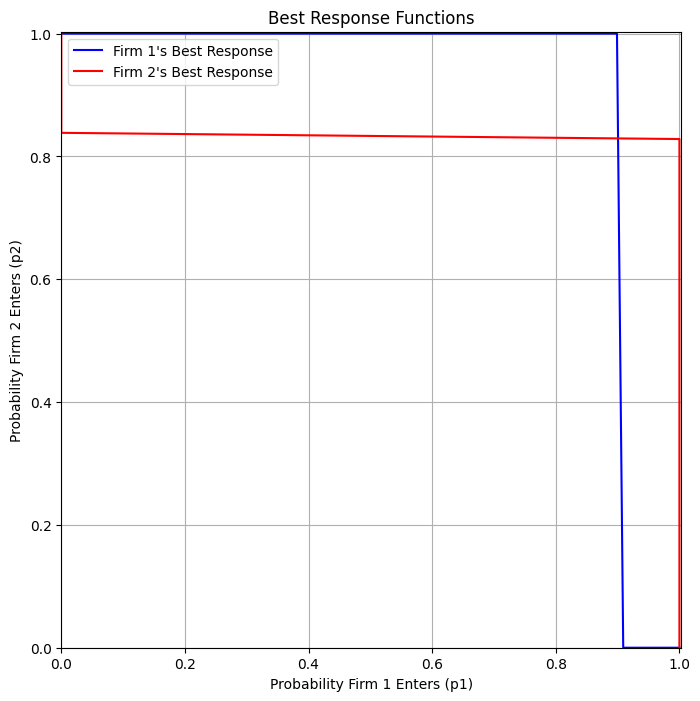
\includegraphics{/workspaces/TexFile/Microeconomic/graph/5.3.3.png}}
 \caption{Best Response Functions}
 \label{}
\end{figure}

$\text { The mixed-strategy equilibrium is }\left(p_{1}^{*}, 1-p_{1}^{*}\right) ;\left(p_{2}^{*}, 1-p_{2}^{*}\right)=(5 / 6,1 / 6) ;(10 / 11,1 / 11) \text {. }$
\item Given the best response functions:

- If Firm 1 believes that Firm 2 will enter with a probability greater than or equal to \(\frac{10}{11}\), Firm 1 will choose not to enter.

- If Firm 2 believes that Firm 1 will enter with a probability greater than or equal to \(\frac{5}{6}\), Firm 2 will choose not to enter.

Considering these best responses, a mixed-strategy Nash equilibrium would involve both firms randomizing their entry decisions based on the above probabilities.

However, if we were to pick a more plausible equilibrium from the pure strategies, it would be one where only one of the firms enters the market, given the high profits for unilateral entry and the losses when both enter. Which firm enters would depend on external factors not captured in the game matrix, such as firm-specific advantages, market research, or prior experience in similar markets.
\end{enumerate}
\end{document}